% --------------------------------------------------------------------------- %
% Poster for the ECCS 2011 Conference about Elementary Dynamic Networks.      %
% --------------------------------------------------------------------------- %
% Created with Brian Amberg's LaTeX Poster Template. Please refer for the     %
% attached README.md file for the details how to compile with `pdflatex`.     %
% --------------------------------------------------------------------------- %
% $LastChangedDate:: 2011-09-11 10:57:12 +0200 (V, 11 szept. 2011)          $ %
% $LastChangedRevision:: 128                                                $ %
% $LastChangedBy:: rlegendi                                                 $ %
% $Id:: poster.tex 128 2011-09-11 08:57:12Z rlegendi                        $ %
% --------------------------------------------------------------------------- %
\documentclass[a0paper,portrait]{baposter}

\usepackage{relsize}		% For \smaller
\usepackage{url}			% For \url
\usepackage{epstopdf}	% Included EPS files automatically converted to PDF to include with pdflatex
\usepackage{epsf,latexsym,amsfonts,amsbsy}
\usepackage{cite}
\usepackage{amsmath, amssymb, amsthm,amscd,amsxtra,amsfonts,bm}
%%% Global Settings %%%%%%%%%%%%%%%%%%%%%%%%%%%%%%%%%%%%%%%%%%%%%%%%%%%%%%%%%%%

\graphicspath{{pix/}}	% Root directory of the pictures
\tracingstats=2			% Enabled LaTeX logging with conditionals

%%% Color Definitions %%%%%%%%%%%%%%%%%%%%%%%%%%%%%%%%%%%%%%%%%%%%%%%%%%%%%%%%%
\DeclareMathOperator*{\argmin}{arg\,min}
\definecolor{bordercol}{RGB}{40,40,40}
\definecolor{headercol1}{RGB}{186,215,230}
\definecolor{headercol2}{RGB}{80,80,80}
\definecolor{headerfontcol}{RGB}{0,0,0}
\definecolor{boxcolor}{RGB}{186,215,230}
\definecolor{blue}{rgb}{0,0,.65}
\definecolor{myblue}{rgb}{0,0,.5}
\definecolor{mygreen}{rgb}{0,.5,0}
\definecolor{red}{rgb}{1,0,0}
\definecolor{myred}{rgb}{.5,0,0}

\newtheorem{dingyi}{Definition~}[section]
\newtheorem{dingli}{Theorem~}[section]
\newtheorem{yinli}{Lemma~}[section]
\newtheorem{tuilun}{Corollary~}[section]
\newtheorem{mingti}{Proposition~}[section]
\newtheorem{caixiang}{Hypothesis~}[section]
\newtheorem{jiashe}{Assumption~}[section]
\newtheorem{lizi}{Instance~}[section]
\newcommand{\zz}{^{\mathrm{T}}}
\newcommand{\fzz}{^{-\mathrm{T}}}
\newcommand{\ff}{_{\mathrm{F}}}
\newcommand{\fs}{^2_{\mathrm{F}}}
\newcommand{\eproof}{$\quad \Box$}
\newcommand{\mR}{\mathbb{R}}
\newcommand{\R}{\mathbb{R}}
\newcommand{\st}{\;\mathrm{s.t.}\;}
\newcommand{\bT}{\mathbb{T}}
\newcommand{\Lone}{\Lambda_1}
\newcommand{\Ltwo}{\Lambda_2}
\newcommand{\Li}{\Lambda_i}
\newcommand{\LA}{\mathcal{L}_{(\beta_1,\ \beta_2)}}
\newcommand{\Po}{\mathcal{P}_\Omega}
\newcommand{\Pob}{\mathcal{P}_{\Omega^c}}
\newcommand{\Zo}{Z_{\omega}}
\newcommand{\La}{\mathcal{L}_{\alpha}}
\newcommand{\bw}{\mathbf{w}}
\newcommand{\bh}{\mathbf{h}}
\newcommand{\Lb}{\mathcal{L}_{\beta}}
%%%%%%%%%%%%%%%%%%%%%%%%%%%%%%%%%%%%%%%%%%%%%%%%%%%%%%%%%%%%%%%%%%%%%%%%%%%%%%%%
%%% Utility functions %%%%%%%%%%%%%%%%%%%%%%%%%%%%%%%%%%%%%%%%%%%%%%%%%%%%%%%%%%

%%% Save space in lists. Use this after the opening of the list %%%%%%%%%%%%%%%%
\newcommand{\compresslist}{
	\setlength{\itemsep}{1pt}
	\setlength{\parskip}{0pt}
	\setlength{\parsep}{0pt}
}

%%%%%%%%%%%%%%%%%%%%%%%%%%%%%%%%%%%%%%%%%%%%%%%%%%%%%%%%%%%%%%%%%%%%%%%%%%%%%%%
%%% Document Start %%%%%%%%%%%%%%%%%%%%%%%%%%%%%%%%%%%%%%%%%%%%%%%%%%%%%%%%%%%%
%%%%%%%%%%%%%%%%%%%%%%%%%%%%%%%%%%%%%%%%%%%%%%%%%%%%%%%%%%%%%%%%%%%%%%%%%%%%%%%

\begin{document}
\typeout{Poster rendering started}

%%% Setting Background Image %%%%%%%%%%%%%%%%%%%%%%%%%%%%%%%%%%%%%%%%%%%%%%%%%%
\background{
	\begin{tikzpicture}[remember picture,overlay]%
	\draw (current page.north west)+(-2em,2em) node[anchor=north west]
	{
\includegraphics[height=1.1\textheight]{background}};
	\end{tikzpicture}
}

%%% General Poster Settings %%%%%%%%%%%%%%%%%%%%%%%%%%%%%%%%%%%%%%%%%%%%%%%%%%%
%%%%%% Eye Catcher, Title, Authors and University Images %%%%%%%%%%%%%%%%%%%%%%
\begin{poster}{
	grid=false,
	% Option is left on true though the eyecatcher is not used. The reason is
	% that we have a bit nicer looking title and author formatting in the headercol
	% this way
	%eyecatcher=false,
	borderColor=bordercol,
	headerColorOne=headercol1,
	headerColorTwo=headercol2,
	headerFontColor=headerfontcol,
	% Only simple background color used, no shading, so boxColorTwo isn't necessary
	boxColorOne=cyan!8!white,
	headershape=roundedright,
	headerfont=\Large\sf\bf,
	textborder=rectangle,
	background=none,
	headerborder=open,
    boxshade=plain
}
%%% Eye Cacther %%%%%%%%%%%%%%%%%%%%%%%%%%%%%%%%%%%%%%%%%%%%%%%%%%%%%%%%%%%%%%%
{
	Eye Catcher, empty if option eyecatcher=false - unused
}
%%% Title %%%%%%%%%%%%%%%%%%%%%%%%%%%%%%%%%%%%%%%%%%%%%%%%%%%%%%%%%%%%%%%%%%%%%
{\sf\bf
	Alternating direction method of multiplier:\\ a powerful tool for difficult optimization problems
}
%%% Authors %%%%%%%%%%%%%%%%%%%%%%%%%%%%%%%%%%%%%%%%%%%%%%%%%%%%%%%%%%%%%%%%%%%
{
	\vspace{1mm} {\smaller Xin Liu (liuxin@lsec.cc.ac.cn)\\  State Key Laboratory of Scientific and Engineering Computing\\
Academy of Mathematics and Systems Science,
Chinese Academy of Sciences}
}
%%% Logo %%%%%%%%%%%%%%%%%%%%%%%%%%%%%%%%%%%%%%%%%%%%%%%%%%%%%%%%%%%%%%%%%%%%%%
{
% The logos are compressed a bit into a simple box to make them smaller on the result
% (Wasn't able to find any bigger of them.)
\setlength\fboxsep{0pt}
\setlength\fboxrule{0.5pt}
	\fbox{
		\begin{minipage}{6.5em}
			%
\includegraphics[width=10em,height=4em]{colbud_logo}
			%
\includegraphics[width=4em,height=4em]{elte_logo} \\
			%
\includegraphics[width=10em,height=4em]{dynanets_logo}
			%
\includegraphics[width=4em,height=4em]{aitia_logo}
            
\includegraphics{tinylogo}
		\end{minipage}
	}
}

\headerbox{Brief Introduction}{name=introduction,column=0,row=0}{
{\color{blue} Philosophy of ADMM}\\
An ancient strategy: {\bf divide} and {\bf conquer}\\
Mathematical view: {\bf split} and {\bf alternate}\\
{\color{blue} Optimization model description}\\
\vspace{-5mm}
\begin{eqnarray*}
\min\limits_{x\in\Omega} f(x) \quad ~\st~ c(x) = 0,
\end{eqnarray*}
with a splitting structure:\\[1mm]
%\begin{itemize}
\indent\qquad $\bullet$ $x:=(x_1,x_2,...,x_p)$\\
\indent\qquad $\bullet$ $\{x\mid x\in\Omega\}=\bigcap\limits_{i=1}^p \{x\mid x_i\in\Omega_i\}$\\
%\end{itemize}
* Split variables are connected by equality constraints.
}

\headerbox{Algorithm Framework}{name=algorithm,column=0,below=introduction}{
Augmented Lagrangian function {\color{purple}(Henstenes 1969, Powell 1969, Rockafellar
1973)}
\begin{eqnarray*}
\Lb(x,\lambda) = f(x) - \lambda\zz c(x) +
\frac{\beta}{2}||c(x)||^2_2.
\end{eqnarray*}

Alternating direction method of multiplier (ADMM)
{\color{purple}(Glowinski-Marocco 1975, Gabay-Mercier
1976, $p=2$, ...)}
\begin{eqnarray*}
\left\{
  \begin{array}{ll}
    {\color{myblue}x_1^{k+1}} \gets \argmin\limits_{\color{red}x_1\in \Omega_1}
     \Lb({\color{red}x_1},x_2^k,...,x_p^k,\lambda^k); \smallskip \\
    {\color{myblue}x_2^{k+1}} \gets \argmin\limits_{\color{red}x_2\in \Omega_2}
    \Lb({\color{mygreen}x_1^{k+1}},{\color{red}x_2},x_3^k,...,x_p^k,\lambda^k); \smallskip \\
    ... ... \smallskip \\
    {\color{myblue}x_p^{k+1}} \gets \argmin\limits_{\color{red}x_p\in \Omega_p}
    \Lb({\color{mygreen}x_1^{k+1}},...,{\color{mygreen}x_{p-1}^{k+1}},{\color{red}x_p},\lambda^k); \smallskip \\
    {\color{myblue}\lambda^{k+1}} \gets \lambda^k - \tau\,\beta\,
    c({\color{mygreen}x_1^{k+1}},...,{\color{mygreen}x_p^{k+1}}).
  \end{array}
\right.
\end{eqnarray*}
}

\headerbox{Convergence}{name=convergence,column=0,below=algorithm}{
{\color{blue} Existent results -- based on strict conditions}\\
\indent $\bullet$ Two blocks, joint convexity, separability {\color{purple}
(Gabay-Mercier 1976)} \\
\indent $\bullet$ Multi-blocks, joint convexity, separability\\
\indent\quad  {\footnotesize $\bullet$ variant versions  {\color{purple}
(He-Yuan et al., Goldfarb-Ma, ...)}} \\
\indent\quad  {\footnotesize $\bullet$ strongly convexity  {\color{purple}
(Luo, 2012)}} \\
\indent $\bullet$ Global linear convergence rate\\
\indent\quad  {\footnotesize $\bullet$ linear programming  {\color{purple}
(Eckstein-Bertsekas, 1990)}} \\
\indent\quad  {\footnotesize $\bullet$ strongly convexity, Lipschitz gradient  {\color{purple}
(Deng-Yin)}} \\
{\color{blue} Nonconvex and nonseparable case} {\color{purple}
(Yang-L.-Zhang)}\cite{YangLiuZhang2012}\\
\indent $\bullet$ Some pioneering results on the local convergence and linear local convergence rate \\
\indent $\bullet$ Milder restriction on the optimization model: the second order sufficiency at the solution\\
}

\headerbox{References}{name=references,column=0,below=convergence}{
\smaller													% Make the whole text smaller
\vspace{-0.4em} 										% Save some space at the beginning
\bibliographystyle{plain}							% Use plain style
\renewcommand{\section}[2]{\vskip 0.05em}		% Omit "References" title
\begin{thebibliography}{1}							% Simple bibliography with widest label of 1
\itemsep=-0.01em										% Save space between the separation
\setlength{\baselineskip}{0.4em}					% Save space with longer lines
\bibitem{YangLiuZhang2012} J. Yang, X. Liu and Y. Zhang.: \emph{A Class of Stationary Iterative Method for Saddle Point
Problems: Convergence and Extension}, finished
\bibitem{WenYangLiu2012} Z. Wen, C. Yang, X. Liu and S.
Marchesini: \emph{Alternating Direction Methods for Classical and
Ptychographic Phase Retrieval}, accepted by Inverse Problem
\bibitem{WenPengLiu2012} Z. Wen, X. Peng, X. Liu, X. Bai and X. Sun: \emph{Asset Allocation under the Basel Accord Risk Measures}, finished
\bibitem{Zhang2010} Y. Zhang: \emph{     An Alternating Direction Algorithm for Nonnegative Matrix Factorization }, Rice technical report, 2010.
\end{thebibliography}
}

\headerbox{Acknowledgements}{name=acknowledgements,column=0,below=references, above=bottom}{
\smaller						% Make the whole text smaller
\vspace{-0.4em}			% Save some space at the beginning
Research supported in part
by NSFC grant 11101409 and 10831006, and the National Center for
Mathematics and Interdisciplinary Sciences, CAS.
}

\headerbox{Ptychographic Phase Retrieval}{name=phaseretrieval,span=2,column=1,row=0}{
\begin{minipage}{70mm}
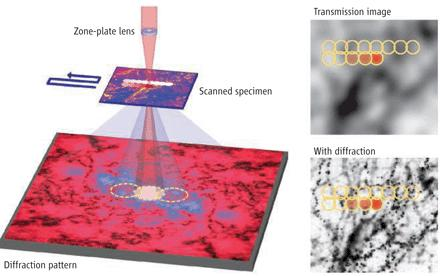
\includegraphics[width=\linewidth,height=42mm]{ptph2.jpg}
\end{minipage}
\hfil
\begin{minipage}{80mm}
\indent $\bullet$  Details refer to {\color{purple}
(Wen-Yang-L.-Marchesini, 2012)}   \cite{WenYangLiu2012} \\[1mm]
%
\indent $\bullet$  Background: X-ray diffractive
imaging, \\
\indent\quad transmission electron microscopy\\[1mm]
%
\indent $\bullet$   Mathematical problem: given $|\mathcal{F} (Q_i \psi)|$ \\
\indent\quad for $i=1,\ldots,k$, can
we recover $\psi$?\\[1mm]
%
\indent $\bullet$ {\color{blue} Optimization model: \color{mygreen} nonconvex, nonsmooth}
\vspace{-2mm}
\begin{eqnarray*}
\min\limits_{\hat \psi\in \mathbb{C}^{n}}\sum_{i=1}^k
\frac{1}{2}\left|\left||\mathcal{F} Q_i \hat \psi| -
b_i\right|\right|_2^2.
\end{eqnarray*}
\end{minipage}
\\[1mm]

{\color{blue} Splitting reformulation:}
$\min\limits_{\hat \psi\in \mathbb{C}^{n}, {\color{red}z\in
\mathbb{C}^{m\times k}}}\sum_{i=1}^k
\frac{1}{2}\left|\left||{\color{red}z_i}| - b_i\right|\right|_2^2
\quad ~\st~  {\color{red}z_i} = \mathcal{F} Q_i \hat \psi, \quad i =
1,...,k.$\\[1mm]
%
{\color{blue} Augmented Lagrangian:}
$\mathcal{L}_{\beta}(z_i,\psi, y_i) = \sum_{i=1}^k \left(\frac{1}{2}
\| |{\color{red}z_i}| - b_i\|_2^2 + y_i^* (\mathcal{F} Q_i \psi -
{\color{red}z_i}) + \frac{\beta}{2}\|\mathcal{F} Q_i \psi -
{\color{red}z_i}\|_2^2 \right).$\\[1mm]
%
{\color{blue} Updating $z$:}  ${\color{red}(z_i^+)_{(l)}}= \left\{\begin{array}{cc}
\frac{|(s_i)_{(l)}|+(b_i)_{(l)}}{(1+\beta)|(s_i)_{(l)}|}(s_i)_{(l)},
& \mbox{if\ }
(s_i)_{(l)}\neq 0 \mbox{\ and\ } (b_i)_{(l)}> 0;  \\
\pm\frac{(b_i)_{(l)}}{1+\beta}, & \mbox{if\ }
(s_i)_{(l)}= 0 \mbox{\ and\ } (b_i)_{(l)}> 0;\\
0, & \mbox{otherwise},\\
\end{array}\right.$ \\
\indent\qquad\qquad\qquad where $s_i = y_i + \beta\mathcal{F} Q_i\psi,\ i=1,...,k$. (closed-form formula)\\[1mm]
%
{\color{blue} Updating $\psi$:} $\psi^+ = \frac{1}{\beta} \left(\sum _{i=1}^k Q_i^* Q_i
\right)^{-1}\sum _{i=1}^k Q_i^* \mathcal{F}^* \left( \beta
{\color{red}z_i^+} - y_i \right).$ (solving linear system)\\[1mm]
%
{\color{blue} Updating Lagrangian multiplier $y$:} $y_i^{j+1}= y_i^j + \tau\,\beta\, (\mathcal{F} Q_i \psi^{j+1} -
{\color{red}z_i^{j+1}}), \quad i = 1, \ldots, k.$
}

\headerbox{Portfolio Optimization}
{name=portfolio,span=2,column=1,below=phaseretrieval}{
\begin{minipage}{68mm}
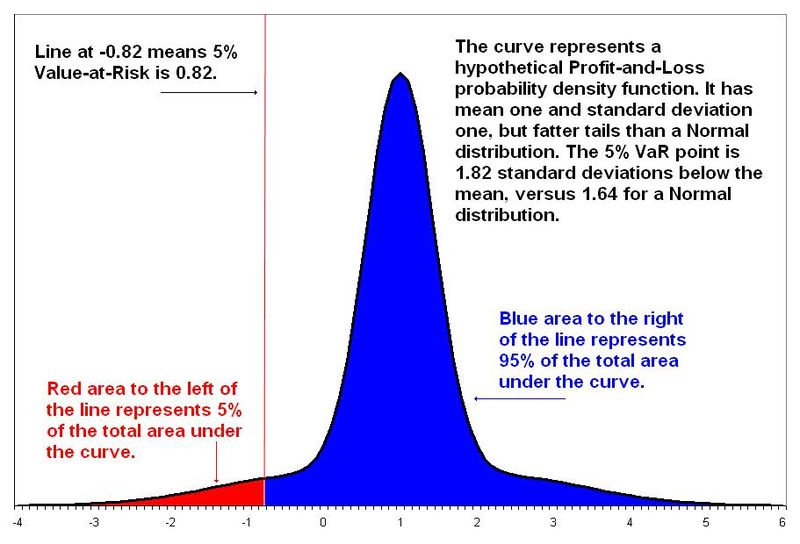
\includegraphics[width=\linewidth,height=42mm]{Var.jpg}
\end{minipage}
\hfil
\begin{minipage}{82mm}
\indent $\bullet$  Details refer to {\color{purple}
(Peng-Wen-L.-Bai-Sun)}   \cite{WenPengLiu2012} \\[1mm]
%
\indent $\bullet$  Value at risk: ${\mathrm{VaR}}_{\alpha}(X) \,\triangleq\, - \inf\limits_{x\in\mR} x
\, ~\st~ \,
{\mathrm{P}}(X>x)\leq$\\
\indent \quad $1-\alpha \,=\, - \inf\limits_{x\in\mR} x \,
~\st~ \, {\mathrm{F}}_X(x)
> \alpha$.\\[1mm]
%
\indent $\bullet$ {\color{blue} Optimization model: \color{mygreen} combinatorial objective}
\vspace{-2mm}
\begin{eqnarray*}
\min\limits_{u\in \mathcal{U}_{r_0}} (-\tilde{R}u)_{(p)},
\end{eqnarray*}
where $\mathcal{U}_{r_0} =\{ u \in \R^d \mid \mu\zz u \geq r_0,
\mathbf{1}\zz u = 1, u \ge 0 \}$; $(\cdot)_{(p)}$ refers to the
$p$-th smallest component of a vector.
\end{minipage}
\\[1mm]

{\color{blue} Splitting reformulation:}
$\min_{ u \in \mathcal{U}_{r_0},  \; {\color{red}x \in \R^n}}
{\color{red}x_{(p)}} \quad ~\st~ {\color{red}x} + \tilde{R}u = 0.$\\[1mm]
%
{\color{blue} Augmented Lagrangian:}
$\Lb(x,u,\lambda):= {\color{red}x_{(p)}} - \lambda\zz ({\color{red}x}
+ \tilde{R} u) + \frac{\beta}{2} \| {\color{red}x} + \tilde{R} u
\|^2.$\\[1mm]
%
{\color{blue} Updating $x$:}  $x_{(i)} = \left\{\begin{array}{ccc} \gamma_{i^*}, &\mbox{if}&
 i^* \leq i\leq p;\\ v_i, && \mbox{otherwise},
\end{array}\right.$ where $v^{(j)} = - \left(\tilde{R} u^{(j)} + \frac{1}{\beta}
\lambda^{(j)} \right)$,  $\gamma_i = \frac{ \beta \sum_{j=i}^p v_j - 1}{ \beta (p-i+1) }$ \\
\indent\qquad\qquad\qquad $i^*:= \max \{ i \mid i\le p, \; v_{i-1} < \gamma_i  \}$ after sorting $ v_1 \le v_2 \le \ldots \le v_n$. (closed-form formula)\\[1mm]
%
{\color{blue} Updating $u$:} $ u^{(j+1)}  =   \argmin_{ u \in \mathcal{U}_{r_0}} \;
 \frac{1}{2} u^\top \tilde{R}^\top \tilde{R} u + b^\top u$, where $b=\tilde{R}^\top (\frac{1}{\beta} \lambda^{(j)}  +
{\color{red}x^{(j+1)}})$ (solving QP)\\[1mm]
%
{\color{blue} Updating Lagrangian multiplier $\lambda$:} $\lambda^{(j+1)} =  \lambda^{(j)} + \beta ({\color{red}x^{(j+1)}}+
\tilde{R} u^{(j+1)}).$
}

\headerbox{Structure Enforcing Matrix
Factorization}
{name=semf,span=2,column=1,below=portfolio,above=bottom}{
\begin{minipage}{48mm}
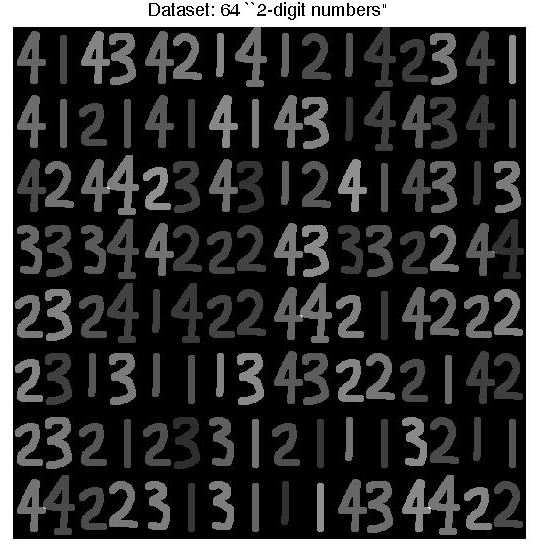
\includegraphics[width=0.93\linewidth,height=43mm]{digit0}
\end{minipage}
\hspace{-5mm}
$\Rrightarrow$
\begin{minipage}{14mm}

\includegraphics[width=0.47\linewidth,height=43mm]{digitPCs}
\end{minipage}
\hspace{-7mm}
\begin{minipage}{92mm}
\indent $\bullet$  Principal component analysis (PCA) with structures: \\
\indent \quad given dataset $A \in\R^{m\times n}$, find $W, H$ with $k\ll n$
columns\\
\indent \quad so that $A \approx WH\zz ~~\Leftrightarrow~~ {\bf a}_j \approx
\bw_1h_{j1} + \bw_2h_{j2} + \cdots + \bw_kh_{jk}.$ \\
\indent \quad with {\color{myred}  prior information} on decomposition pattern $(W,H)$ \\[2mm]
\indent $\bullet$   {\color{blue} Optimization model: \color{mygreen} nonconvex, combinatorial constraints}
\vspace{-6mm}
\begin{eqnarray*}
\min_{W\in\R^{m\times k},\ H\in\R^{n\times k}} \|A - WH\zz\|\fs
~\st~ W \in \bT_1, \; H \in \bT_2,
\end{eqnarray*}
%\footnote{details refer to {\color{purple}
%(Zhang, 2010)}  \cite{Zhang2010}}
where $\bT_1$, $\bT_2$ can be $\{X\mid X\zz X =I\}$, or $\{X \mid
X\geq
0\}$ (nonnegative matrix factorization, {\color{purple}
(Zhang, 2010)}  \cite{Zhang2010}), or any other matrix sets allowing {\color{myred}`easy projection'}.
\end{minipage}
\\[1mm]
\begin{minipage}{85mm}
\indent $\bullet$ {\color{blue} Splitting reformulation:} $\min_{W,\ H,\ {\color{red}S_1},\ {\color{red}S_2}} \|A - WH\zz\|\fs$
\indent \quad $~\st~ W={\color{red}S_1} \in \bT_1, \; H={\color{red}S_2} \in \bT_2.$\\
\indent  $\bullet$  {\color{blue} Augmented Lagrangian:}
$\LA(W,H,{\color{red}S_1},{\color{red}S_2},\Lambda)  = $ \\
\indent \quad $\|A - WH\zz\|\fs - \Lone\bullet(W-{\color{red}S_1}) -
\Ltwo\bullet(H-{\color{red}S_2}) $ \\
\indent \quad $+ \frac{\beta_1}{2}\cdot\|W-{\color{red}S_1}\|\fs +
\frac{\beta_2}{2}\cdot\|H-{\color{red}S_2}\|\fs.$ \\[2mm]
\indent $\bullet$ $\left\{
  \begin{array}{ll}
    W^{k+1} \gets \arg\min_{W} \LA(W,H^k,{\color{red}S_1^k},{\color{red}S_2^k},\Lambda^k); \smallskip \\
    H^{k+1}  \gets \arg\min_{H} \LA(W^{k+1},H,{\color{red}S_1^k},{\color{red}S_2^k},\Lambda^k); \smallskip \\
    {\color{red}S_i^{k+1}}  \gets {\rm Proj}\,_{\bT_i}(V_i^{k+1}-\Li^k/\beta_i); \quad{\color{myred}\mbox{Here,}\, i=1,2; }\smallskip \\
    \Li^{k+1}  \gets \Li^k -  \beta_i(V_i^{k+1}-{\color{red}S_i^{k+1}}). \quad {\color{myred} V_1=W, V_2=H.}
  \end{array}
\right.$
\end{minipage}
\hfil
\begin{minipage}{65mm}
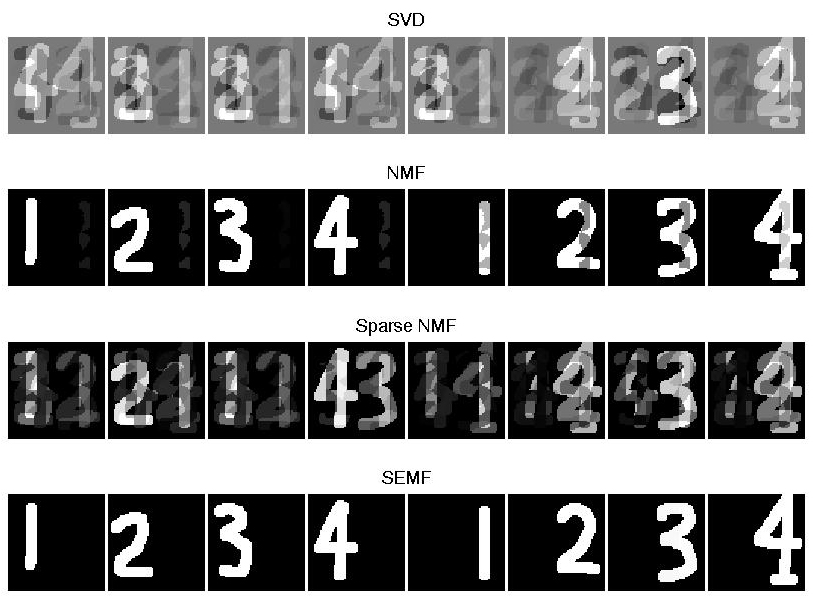
\includegraphics[width=\linewidth,height=42mm]{digit2t.jpg}
\end{minipage}
}

\end{poster}
\end{document}
